%!TEX root = ./Structure_rapport_final.tex

\subsection{Factorial Analysis of Mixed Data}

The first 5 FAMD components explained 80\% of the total variation (Table \ref{table:cont_abs}). The first axis (30.5\% of explained variance) is strongly correlated with shape of the body and of the head with traits such as \emph{body depth} (a = 11.7), \emph{lower jaw length} (a=11.5), \emph{oral gape axis} (a=11.1), orbital length (a = 8.35) and head length (a = 8.21) (Table \ref{table:cont_abs}). Along this axis, all traits have increasing values toward the right (see \ref{fig:corr_circ_12} for details). As can be seen on Figure \ref{fig:famd12}, this axis clearly separates 3 groups of fishes. For low PC1 values, fishes have a low transversal shape (meaning that both \textsc{bd} and \textsc{bw} have similar values, consistent with an elongated body), short lower jaw, small oral gape surface and a terminal oral axis, such as \textit{A. risso}, \textit{S. boa} and \textit{S. beanii}. On the right of this axis, fishes display high body depth values suggesting a laterally compressed form and a superior-oriented oral axis, such as \textit{A. olfersii}. 
The second axis (21.6\% of explained variance) is correlated with habitat, through food prospection behaviour with \emph{pectoral fin insertion} (a = 11.4), \emph{eye size} (a = 9, \emph{pectoral fin position} (a = 7.1) and food acquisition through \emph{gill raker type} (a = 17.8) and \emph{oral gape axis} (a = 12,3) (Table \ref{table:cont_abs}). This axis separates the 3 species on the left, \textit{A. risso} and \textit{S. boa} diplay higher values of pectoral fin insertion, meaning that the fin is inserted further on the body than \textit{S. boa}, while the fin position on the body depth is lower. Because \textit{S. beanii} does not have pectoral fin, same analysis has been run without traits refering to pectoral or pelvic fins to look if discrimination between species were highly dependant if these traits. Same results than Figure \ref{fig:famd12} were obtained. Thus, without the entire \textit{S. beanii} species, it seems that \textit{A. risso} and \textit{S. boa} are no longer overlapping. 
The third axis (explaining 12.2\% of total variance) mainly carries traits linked to the diet, with strong influence of \emph{anus position} (a = 23.8), \emph{gill raker type} (a = 19.2), \emph{dorsal fin insertion} (a = 15.5) and \emph{pectoral fin position} (a = 14.2) (Table \ref{table:cont_abs}). On the left of this axis, species are characterized by a rather high pectoral fin insertion and close-to-head dorsal fin insertion and anus position (see Figures \ref{fig:famd34} and \ref{fig:corr_circ_34}).
Finally, the fourth axis (explaining 7.9\% of variance) is mainly related to traits linked to prey selection, with \emph{pyloric caeca} (a = 31.6), \emph{opercumulum volume} (a = 17) and \emph{presence of photophores} (a = 10.9) (Table \ref{table:cont_abs}). The remaining PC scores (20\% of variance) are mainly linked to food acquisition. 
Overall, several species' ellipses are overlapping in both Figure \ref{fig:famd12} and Figure \ref{fig:famd34}. In the first, all 4 Myctophidae and 2 Platytrocidae species, plus \textit{X. copei} are more or less overlapping, not displaying much differences along PC1 nor PC2. On the same figure \textit{A. risso} and \textit{S. boa} seems to slightly overlap each other niches, which are mainly separated along PC2. \textit{S. beanii} and \textit{A. olfersii} are the only two species not showing any overlap. 
In Figure \ref{fig:famd34} \textit{A. risso} and \textit{A. olfersii} are showing some overlap. On the same figure, the same species (except \textit{X. copei}) than Figure \ref{fig:famd12} overlaps. Especially, \textit{N. operosus} and \textit{S. koefoedi} have very similar looking niches, which seems virtually fully overlapping. \textit{L. crocodilus}, which have the widest niche among these species, overlaps \textit{C. maderensis}, \textit{M. punctatum} and \textit{N. kroyeri} niches. 


% Table of contributions of variables for 5 first axis
\begin{table}[ht]
\centering
\caption{Correlation between 5 first PC's component and functional traits. In bold, correlations higher than threshold (4.8)}
\label{table:cont_abs}
\begin{adjustbox}{max width=1.1\textwidth,center}
\begin{tabular}{rrrrrr}
  \hline
 & PC1 (30.5\%) & PC2 (21.6\%) & PC3 (12.2\%) & PC4 (7.9\%) & PC5 (7.8\%) \\ 
  \hline
  Eye size & 1.29 & \textbf{9.01} & 3.52 & 4.08 & 1.40 \\ 
  Orbital length & \textbf{8.35} & 2.38 & 0.00 & 2.24 & 4.54 \\ 
  Oral gape surface & \textbf{7.78} & 3.06 & 2.93 & 0.10 & 2.78 \\ 
  Oral gape shape & 0.18 & 3.10 & 0.05 & \textbf{9.49} & \textbf{10.41} \\ 
  Oral gape position & 0.42 & 1.21 & 1.99 & \textbf{9.16} & 3.94 \\ 
  Lower jaw length & \textbf{11.52} & 0.00 & 0.04 & 1.97 & 2.44 \\ 
  Gill outflow & \textbf{5.47} & 0.82 & 0.02 & 2.22 & \textbf{22.48} \\ 
  Operculum volume & 2.52 & 0.03 & 1.61 & \textbf{17.02} & \textbf{5.68} \\ 
  Head length & \textbf{8.21} & 3.10 & 2.50 & 0.78 & 4.50 \\ 
  Anus position & 0.00 & \textbf{5.28} & \textbf{23.81} & 0.07 & 0.77 \\ 
  Body depth & \textbf{11.68} & 0.93 & 1.41 & 0.64 & 1.92 \\ 
  Pectoral fin position & 1.72 & \textbf{7.15} & \textbf{14.22} & 0.37 & 0.32 \\ 
  Pectoral fin insertion & \textbf{4.95} & \textbf{11.39} & 0.05 & 0.12 & 0.74 \\ 
  Transversal shape & \textbf{5.96} & 4.33 & 5.45 & 1.70 & 2.10 \\ 
  Caudal throttle width & 3.72 & \textbf{5.01} & 0.28 & 1.60 & \textbf{16.30} \\ 
  Dorsal fin insertion & 2.58 & 4.78 & \textbf{15.52} & 0.00 & 1.33 \\ 
  Eye position & 0.19 & \textbf{5.41} & 0.78 & 2.34 & 1.40 \\ 
  Oral gape axis & \textbf{11.07} & \textbf{12.28} & 3.32 & 3.27 & \textbf{7.13} \\ 
  Gill raker type & 4.38 & \textbf{17.80} & \textbf{19.23} & 0.32 & 3.42 \\ 
  Pyloric caeca & 0.23 & 0.48 & 0.04 & \textbf{31.62} & \textbf{5.81} \\ 
  Presence photophores & \textbf{7.79} & 2.45 & 3.23 & \textbf{10.89} & 0.59 \\  \\ 
   \hline
\end{tabular}
\end{adjustbox}
\end{table}

% Plot of FAMD axis 1 and 2
\begin{figure} [!htbp]
	\begin{center}
		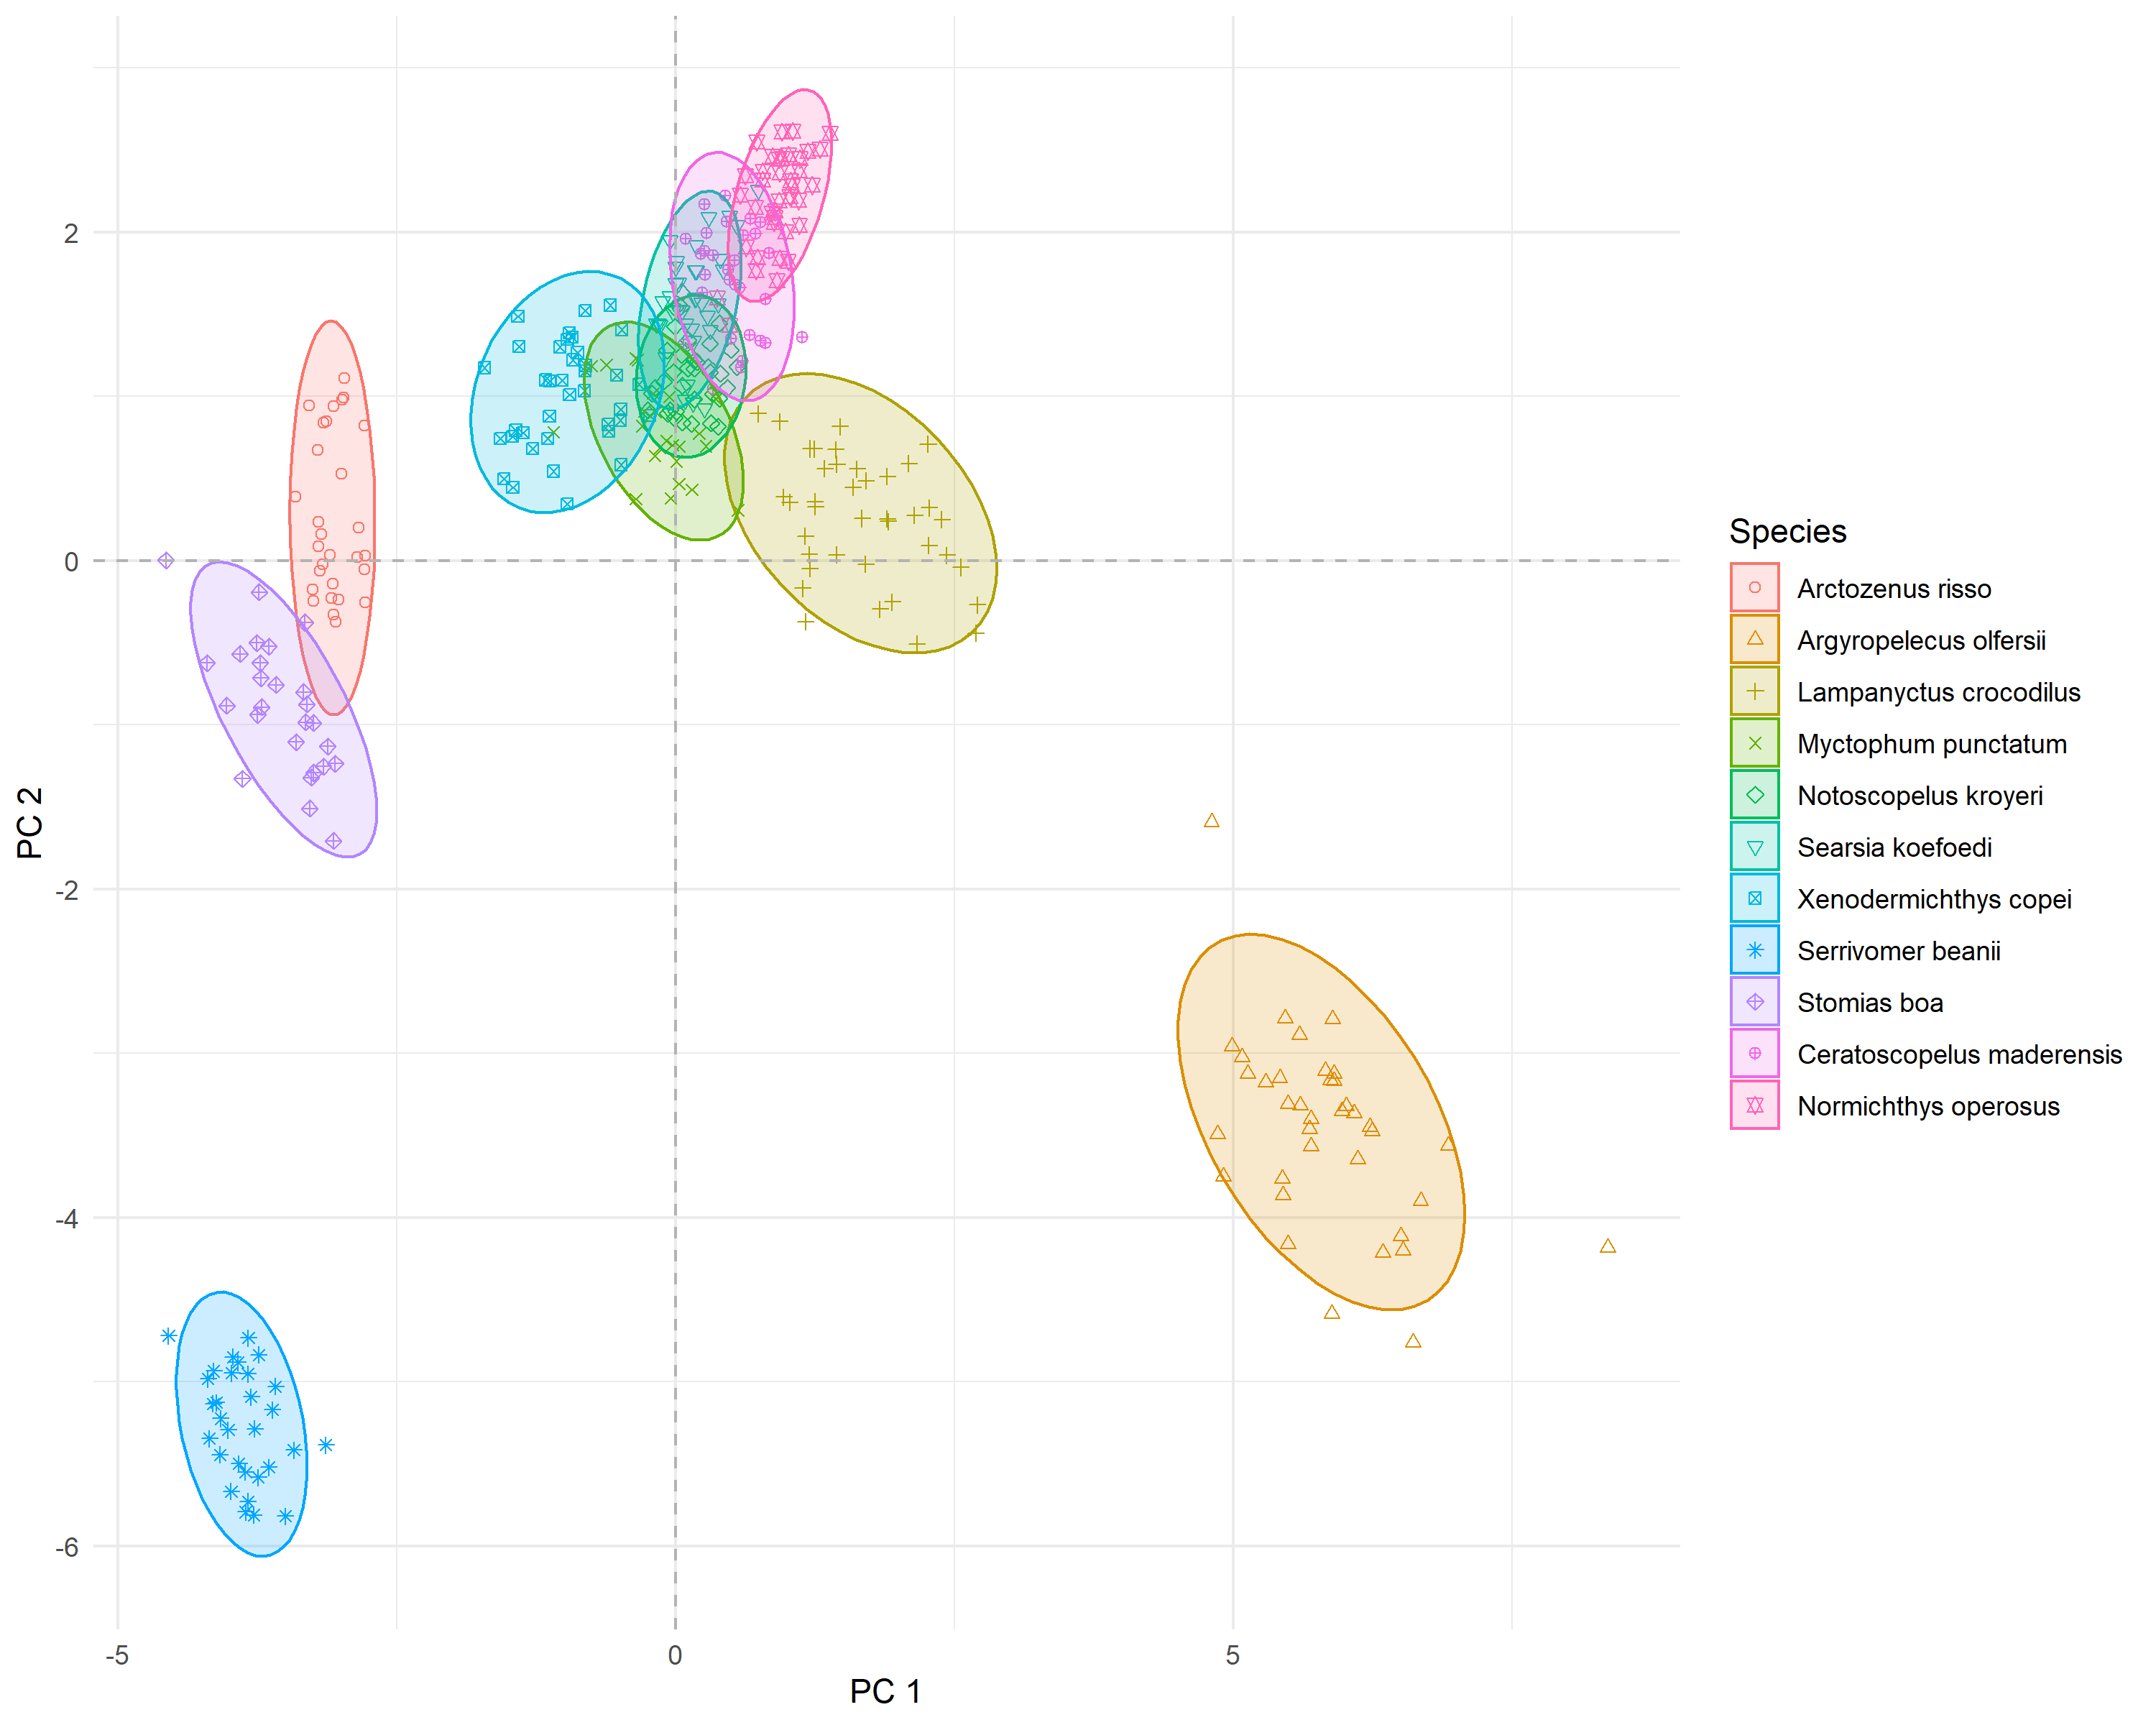
\includegraphics[width=\textwidth]{FAMD_1_2.png}
	\end{center}
	\caption{FAMD results for PC 1 and 2.}
	\label{fig:famd12}
\end{figure}

% Plot of FAMD axis 3 and 4
\begin{figure} [!htbp]
	\begin{center}
		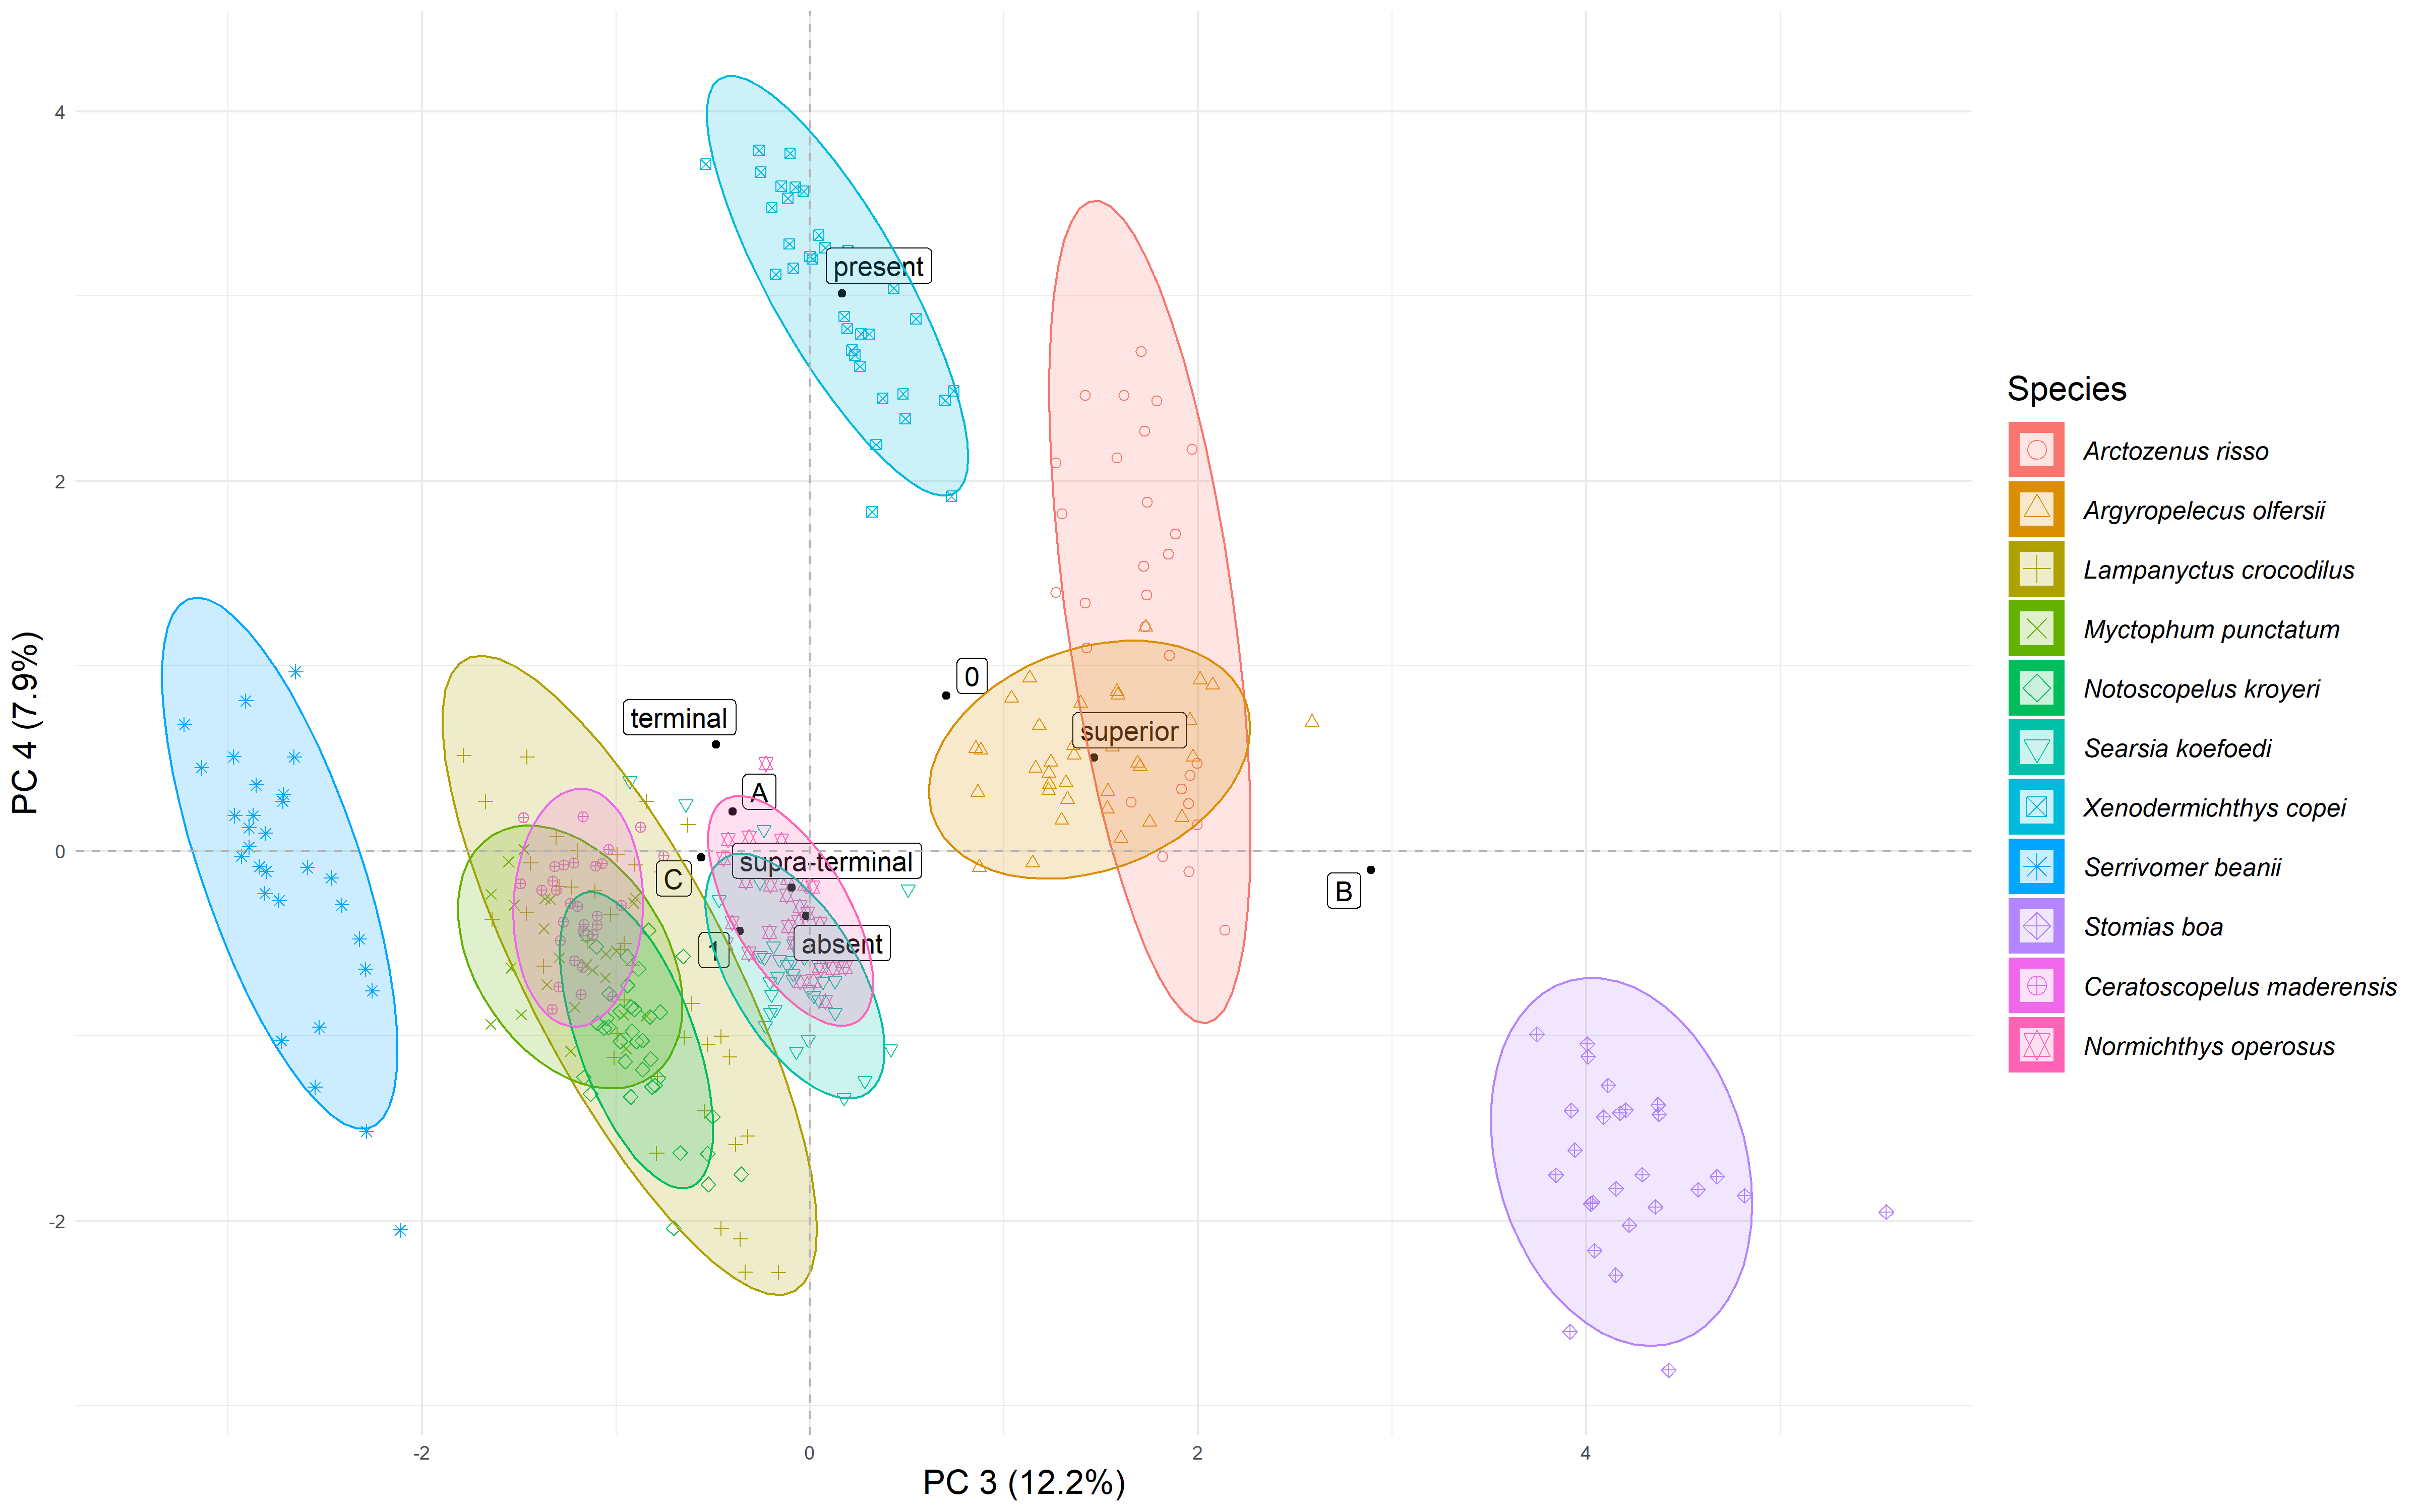
\includegraphics[width=\textwidth]{FAMD_3_4.png}
	\end{center}
	\caption{FAMD results for PC 3 and 4.}
	\label{fig:famd34}
\end{figure}


\subsection{Functional niche area and overlap}
The niche area estimation showed that \textit{N. kroyeri} had the smallest niche, with \textit{N. operosus} and \textit{S. koeoedi} having slightly bigger ones (Table \ref{table:sp_area}). In fact, all Myctophidae (except \textit{L. crocodilus}) and Platytrocidae have rather small niches and are the one overlapping in Figure \ref{fig:famd12}. Conversely, \textit{A. olfersii} is the species with the biggest niche, more than 7 times wider than \textit{N. kroyeri}.
Boostrapped niche area estimation function did not show any difference in the surface of estimated niche through sample size \textit{n}. Areas values seems to be more influenced by the individuals sampled for estimation rather than the number of inviduals itself. Yet, estimated niche area value are tightly converging for \textit{n} = 30. 

% Niche standardardised areas
\begin{table}[ht]
\centering
\caption{Standardized area of functional niches.}
\label{table:sp_area}
\begin{adjustbox}{max width=1.1\textwidth,center}
\begin{tabular}{lr}
  \hline
Species & Area \\ 
  \hline
Argyropelecus olfersii & 7.39 \\ 
  Lampanyctus crocodilus & 4.00 \\ 
  Xenodermichthys copei & 2.60 \\ 
  Stomias boa & 2.54 \\ 
  Myctophum punctatum & 2.13 \\ 
  Serrivomer beanii & 1.89 \\ 
  Arctozenus risso & 1.78 \\ 
  Ceratoscopelus maderensis & 1.75 \\ 
  Searsia koefoedi & 1.33 \\ 
  Normichthys operosus & 1.18 \\ 
  Notoscopelus kroyeri & 1.00 \\ 
   \hline
\end{tabular}
\end{adjustbox}
\end{table}

Niche overlap analysis confirms that 9 species have overlapping niches in Figure \ref{fig:famd12}and that smallest niches overlaps each other the most (Table \ref{table:ell_ovlp}). The maximum  overlap is found between \textit{M. punctatum} and \textit{N. kroyeri}, as almost 69\% of the latter's niche is covered by the first. In total, these two species share nearly 22\% of their niches. Same observation is made between \textit{S. koefoei} whose niche is 65\% covered by \textit{C. maderensis}. These two species have the highest total overlap value, with 28\% of their niches overlapping. Finally, \textit{N. kroyeri} and \textit{N. operosus} show minimum total overlap value of 0.21\%. This is due to some individuals of the latter in \textit{N. kroyeri}'s ellipse (see \ref{fig:famd12}). 

PROBLEME CHIFFRE SIGNIF.

\begin{table}[ht]
\centering
\caption{Species niche overlap. All the others comparisons that are not present in this table did not present any overlap.}
\label{table:ell_ovlp}
\begin{adjustbox}{max width=1.1\textwidth,center}
\begin{tabular}{llrrr}
  \hline
Species1 & Species2 & Overlap of Species 2 over Species 1 (\%) & Overlap of Species 1 over Species 2 (\%) & Total overlap (\%)\\ 
  \hline
Searsia koefoedi & Ceratoscopelus maderensis & 65.44 & 49.64 & 28.23 \\ 
  Notoscopelus kroyeri & Searsia koefoedi & 65.38 & 49.17 & 28.06 \\ 
  Myctophum punctatum & Notoscopelus kroyeri & 32.28 & 68.69 & 21.96 \\ 
  Myctophum punctatum & Xenodermichthys copei & 44.86 & 36.64 & 20.17 \\ 
  Ceratoscopelus maderensis & Normichthys operosus & 31.77 & 47.10 & 18.97 \\ 
  Notoscopelus kroyeri & Ceratoscopelus maderensis & 41.58 & 23.72 & 15.11 \\ 
  Myctophum punctatum & Searsia koefoedi & 20.27 & 32.44 & 12.48 \\ 
  Searsia koefoedi & Normichthys operosus & 15.02 & 16.89 & 7.95 \\ 
  Notoscopelus kroyeri & Xenodermichthys copei & 22.93 & 8.80 & 6.36 \\ 
  Searsia koefoedi & Xenodermichthys copei & 17.47 & 8.92 & 5.90 \\ 
  Lampanyctus crocodilus & Myctophum punctatum & 6.49 & 12.20 & 4.24 \\ 
  Arctozenus risso & Stomias boa & 9.41 & 6.60 & 3.88 \\ 
  Myctophum punctatum & Ceratoscopelus maderensis & 5.78 & 7.01 & 3.17 \\ 
  Lampanyctus crocodilus & Ceratoscopelus maderensis & 2.50 & 5.70 & 1.74 \\ 
  Lampanyctus crocodilus & Notoscopelus kroyeri & 1.20 & 4.79 & 0.96 \\ 
  Notoscopelus kroyeri & Normichthys operosus & 0.46 & 0.39 & 0.21 \\ 
   \hline
\end{tabular}
\end{adjustbox}
\end{table}

Finally, looking at niches' dissimilarities confirms what can be seen on previous figures, which is that all Myctophidae and Platytrocidae species studied here have rather similar niches. Conversely, \textit{A. olfersii}, \textit{S. beanii} and \textit{S. boa} tend to have more distincts niches, which are consistent results with what can be seen on Figure \ref{fig:famd12}. Here, species with the most atypical morphological feature are the more distinct in terms of niche. 

\begin{table}[ht]
\centering
\caption{Niche dissimilarity of studied species}
\label{table:nich_diss}
\begin{adjustbox}{max width=1.1\textwidth,center}
\begin{tabular}{lr}
  \hline
Species & Distinctiveness value \\ 
  \hline
Argyropelecus olfersii & 0.54 \\ 
  Serrivomer beanii & 0.51 \\ 
  Stomias boa & 0.46 \\ 
  Arctozenus risso & 0.40 \\ 
  Lampanyctus crocodilus & 0.37 \\ 
  Xenodermichthys copei & 0.37 \\ 
  Ceratoscopelus maderensis & 0.31 \\ 
  Normichthys operosus & 0.31 \\ 
  Notoscopelus kroyeri & 0.30 \\ 
  Searsia koefoedi & 0.29 \\ 
  Myctophum punctatum & 0.29 \\  
   \hline
\end{tabular}
\end{adjustbox}
\end{table}


\subsection{Kernel density estimation}
The estimation of kernel density overlap for functional traits of the 7 overlapping species of Figure \ref{fig:famd12} and concludes that these species are all overlaping for 7 of the 17 computed traits (see figure \ref{fig:dpo}). The overlap is maximum for the position of the oral gape (trait n°5) with an overlap value of 0.34. This means that, along this functional trait, these 6 species share nearly 34\% of their density. For this trait, most of the distributions are centered around a range of values of [0.5-0.8], yet \textit{L. crocodilus} display a pretty wide distribution, despite being the most sampled species (see Table \ref{table:spcount}). This same observation can be done for this particular species for traits n°11 (body depth) and n°13 (pectoral fin insertion). Species also share nearly 25\% and 29\% of their density when looking at body depth (trait n°11) and eye position (trait n°17), respectively. Finally, lower jaw length (trait n°6) and pectoral fin position (trait n°12) values also seem to be common to those species, with 16\% and 19\% of density shared, respectively. To a lesser extent, species share nearly 12\% of the eye size values (trait n°2).
On most plots of Figure \ref{fig:dpo}, \textit{N. kroyeri} and \textit{M. punctatum} have very similar distributions. When looking at these 2 species only, analysis show that they are overlapping for every 17 traits, with particularly high values for eye size (o = 0.915), gill outflow (o = 0.882), operculum volume (o = 0.901), pectoral fin insertion (o = 0.828) and caudal throttle width (o = 0.782). 


\begin{table}[ht]
\centering
\caption{Kernel density overlap values for the 17 computed traits. Values in bold are significant (p < 0.01) and shown in Figure \ref{fig:dpo}.}
\label{table:kern_over_val}
\begin{adjustbox}{max width=1.1\textwidth,center}
\begin{tabular}{lcr}
  \hline
Trait code & Functional trait & Total overlap (o) \\ 
  \hline
1 & Eye size & 0.00 \\ 
  2 & Orbital length & \textbf{0.12} \\ 
  3 & Oral gape surface & 0.00 \\ 
  4 & Oral gape shape &0.00 \\ 
  5 & Oral gape position & \textbf{0.34} \\ 
  6 & Lower jaw length & \textbf{0.16} \\ 
  7 & Gill outflow & 0.00 \\ 
  8 & Operculum volume & 0.00 \\ 
  9 & Head length & 0.00 \\ 
  10 & Anus position & 0.00 \\ 
  11 & Body depth & \textbf{0.25} \\ 
  12 & Pectoral fin position & \textbf{0.20} \\ 
  13 & Pectoral fin insertion & \textbf{0.01} \\ 
  14 & Transversal shape & 0.00 \\ 
  15 & Caudal throttle width & 0.00 \\ 
  16 & Dorsal fin insertion & 0.00 \\ 
  17 & Eye position & \textbf{0.29} \\ 
   \hline
\end{tabular}
\end{adjustbox}
\end{table} 

\begin{figure} [!htbp]
	\begin{center}
		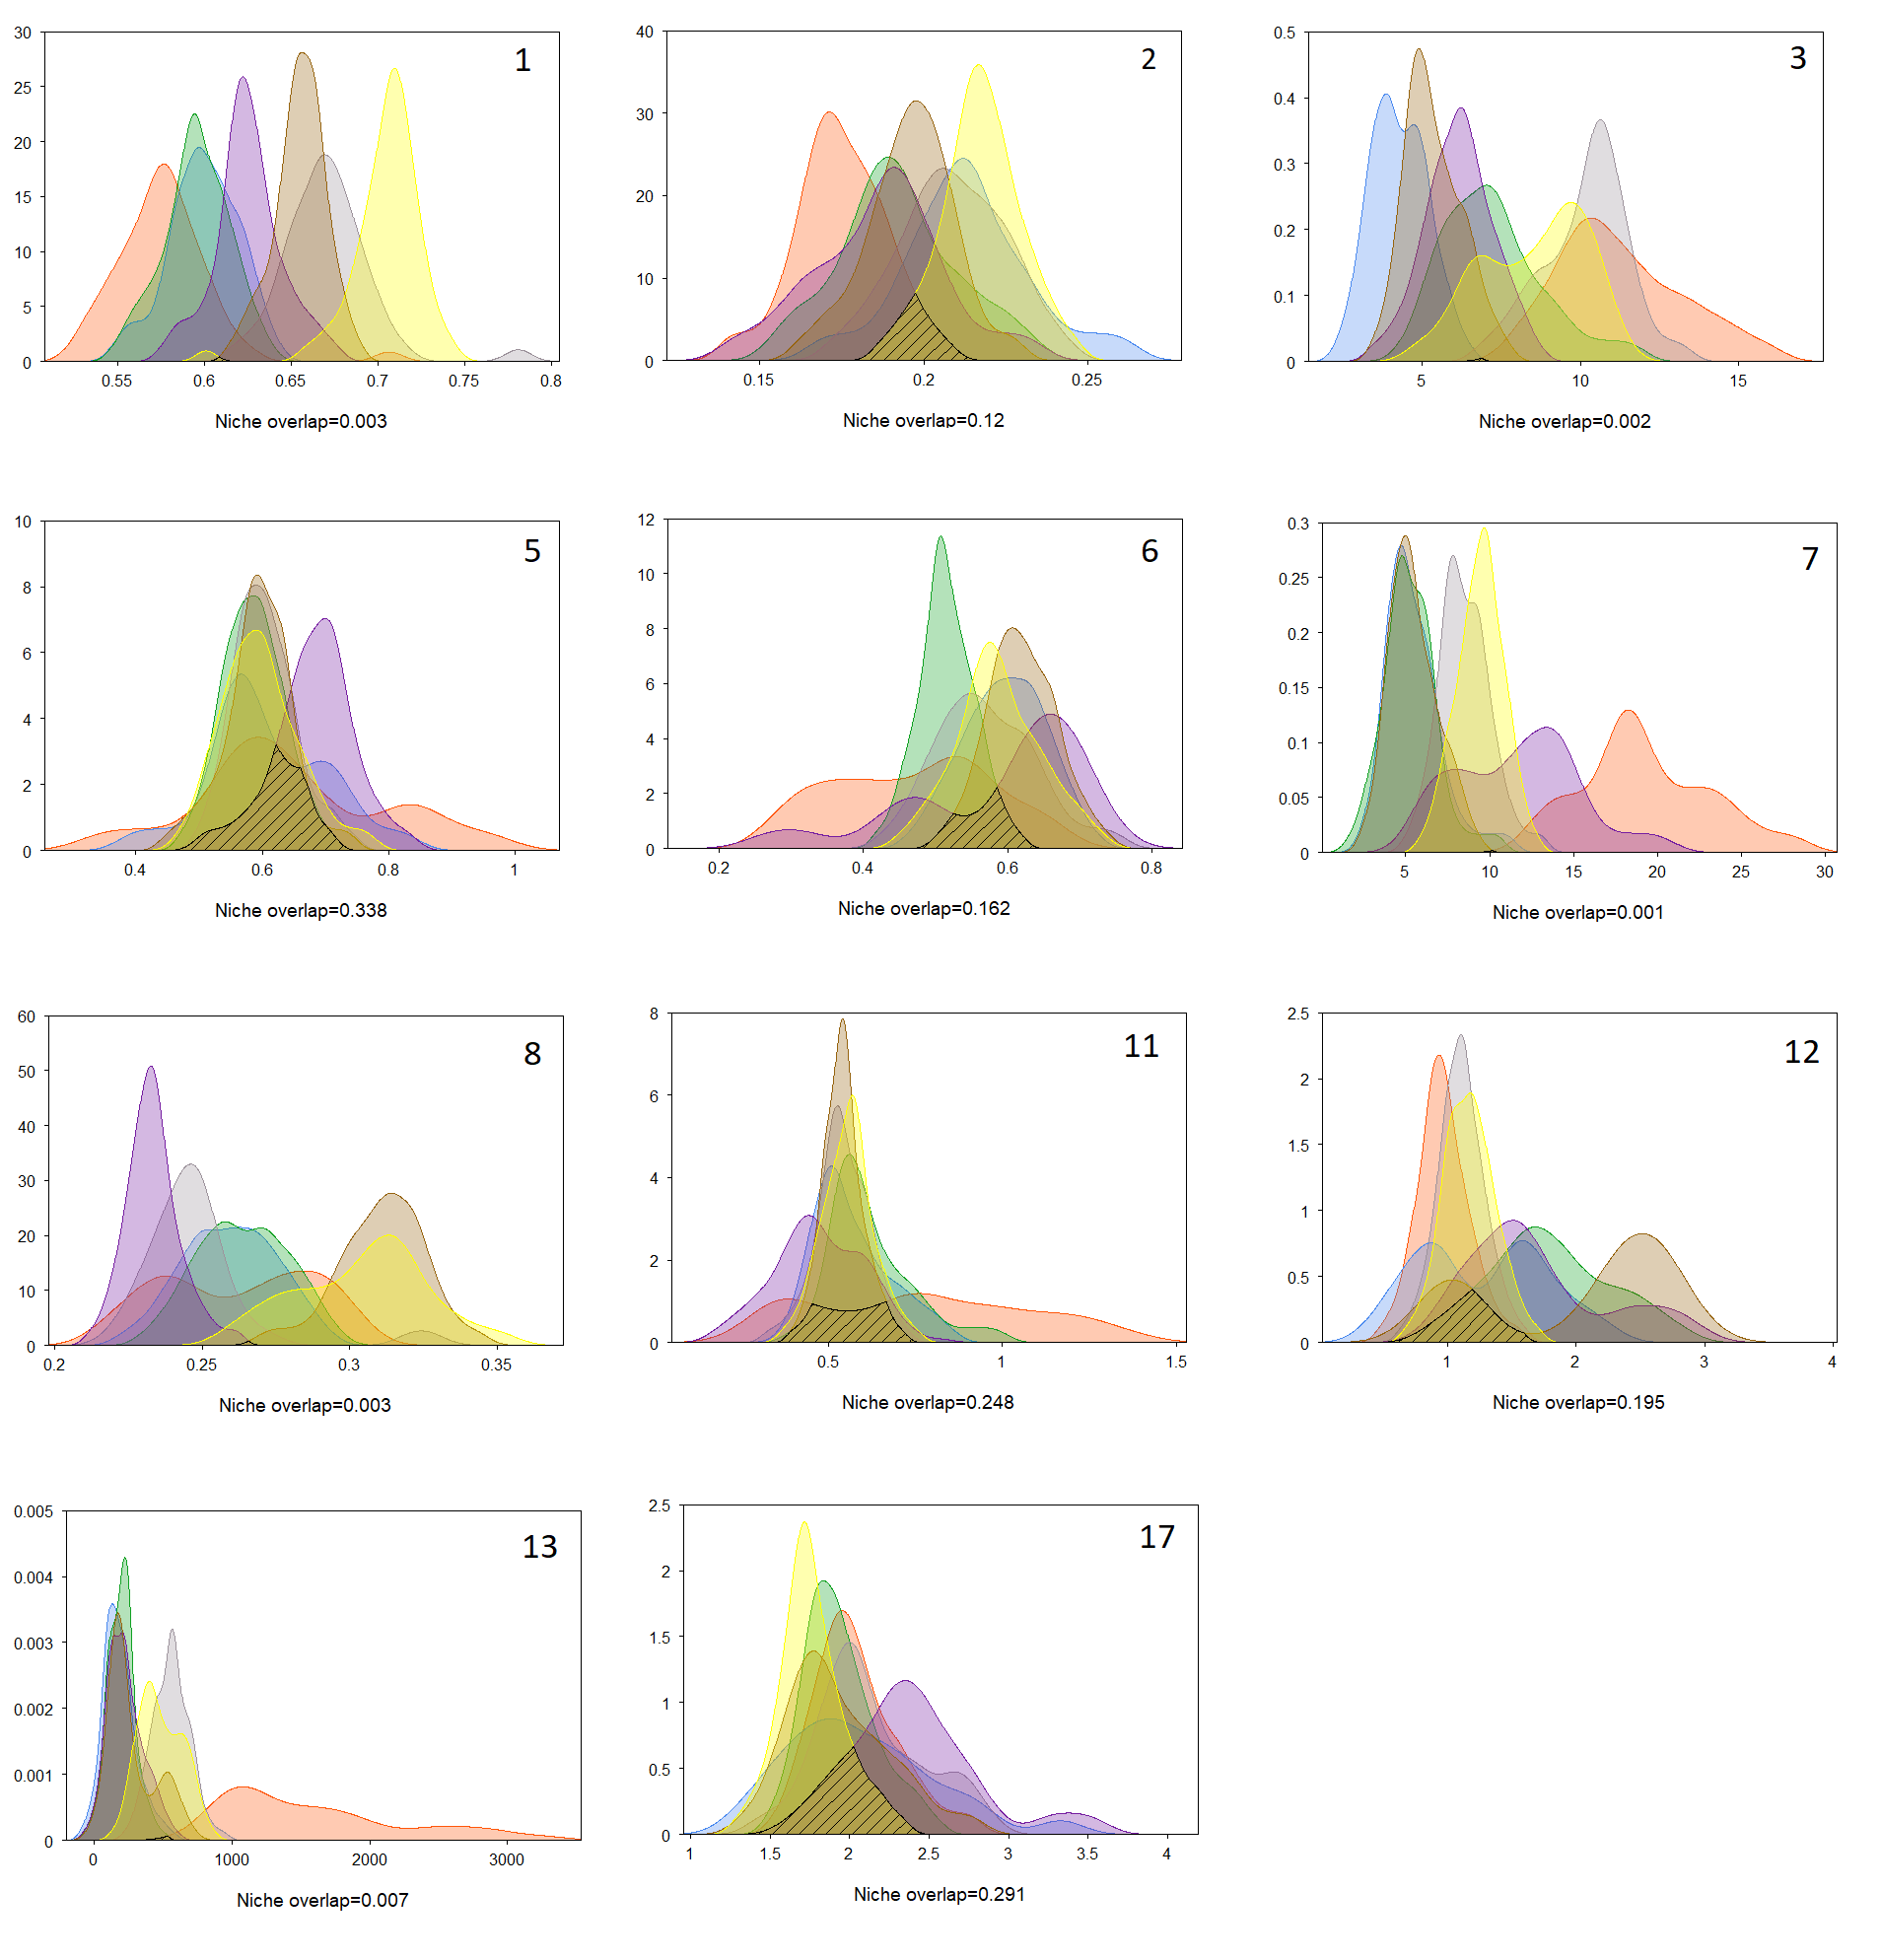
\includegraphics[width=\textwidth]{Density_plot.png}
	\end{center}
	\caption{Kernel density overlap for 11 functional traits and overlaping species. Colors correspond to following species: orange - \textit{L. crocodilus}; brown - \textit{C. maderensis}; yellow - \textit{N. operosus}; purple - \textit{X. copei}; green - \textit{N. kroyeri}; blue - \textit{M. punctatum}; grey - \textit{S. koefoedi}. Here, every traits that showed non-null overlap is displayed.}
	\label{fig:dpo}
\end{figure}